\documentclass[a4paper, DIV12, headsepline]{scrartcl}

% common packages
\usepackage{lmodern}
\usepackage[T1]{fontenc}
\usepackage[utf8]{inputenc}
\usepackage[english]{babel}
\usepackage{amsfonts}
\usepackage{amssymb}
\usepackage{amsmath}
\usepackage{siunitx}
\usepackage{graphicx}
\usepackage{url}
\usepackage{listings}
\usepackage{tikz}
\usepackage{enumitem}
\usepackage[labelfont=bf]{caption}

% set head and foot
\usepackage{scrpage2}
\pagestyle{scrheadings}
\clearscrheadfoot
\ihead{Lab 1 -- Report}
\ohead{Group 25: Hui Jing (cid: huij), Tobias Fuchs (cid: fuchs)}
\cfoot{\pagemark}

% set pdf options
\usepackage[pdfborder={0 0 0}, bookmarksopen=true, bookmarksnumbered=true, pdftitle={Lab 1 Report}, pdfauthor={Hui Jing, Tobias Fuchs}, pdfsubject={Report}]{hyperref}

\begin{document}

\section*{Report for Lab 1}
\subsection*{Task 1}
\begin{center}
	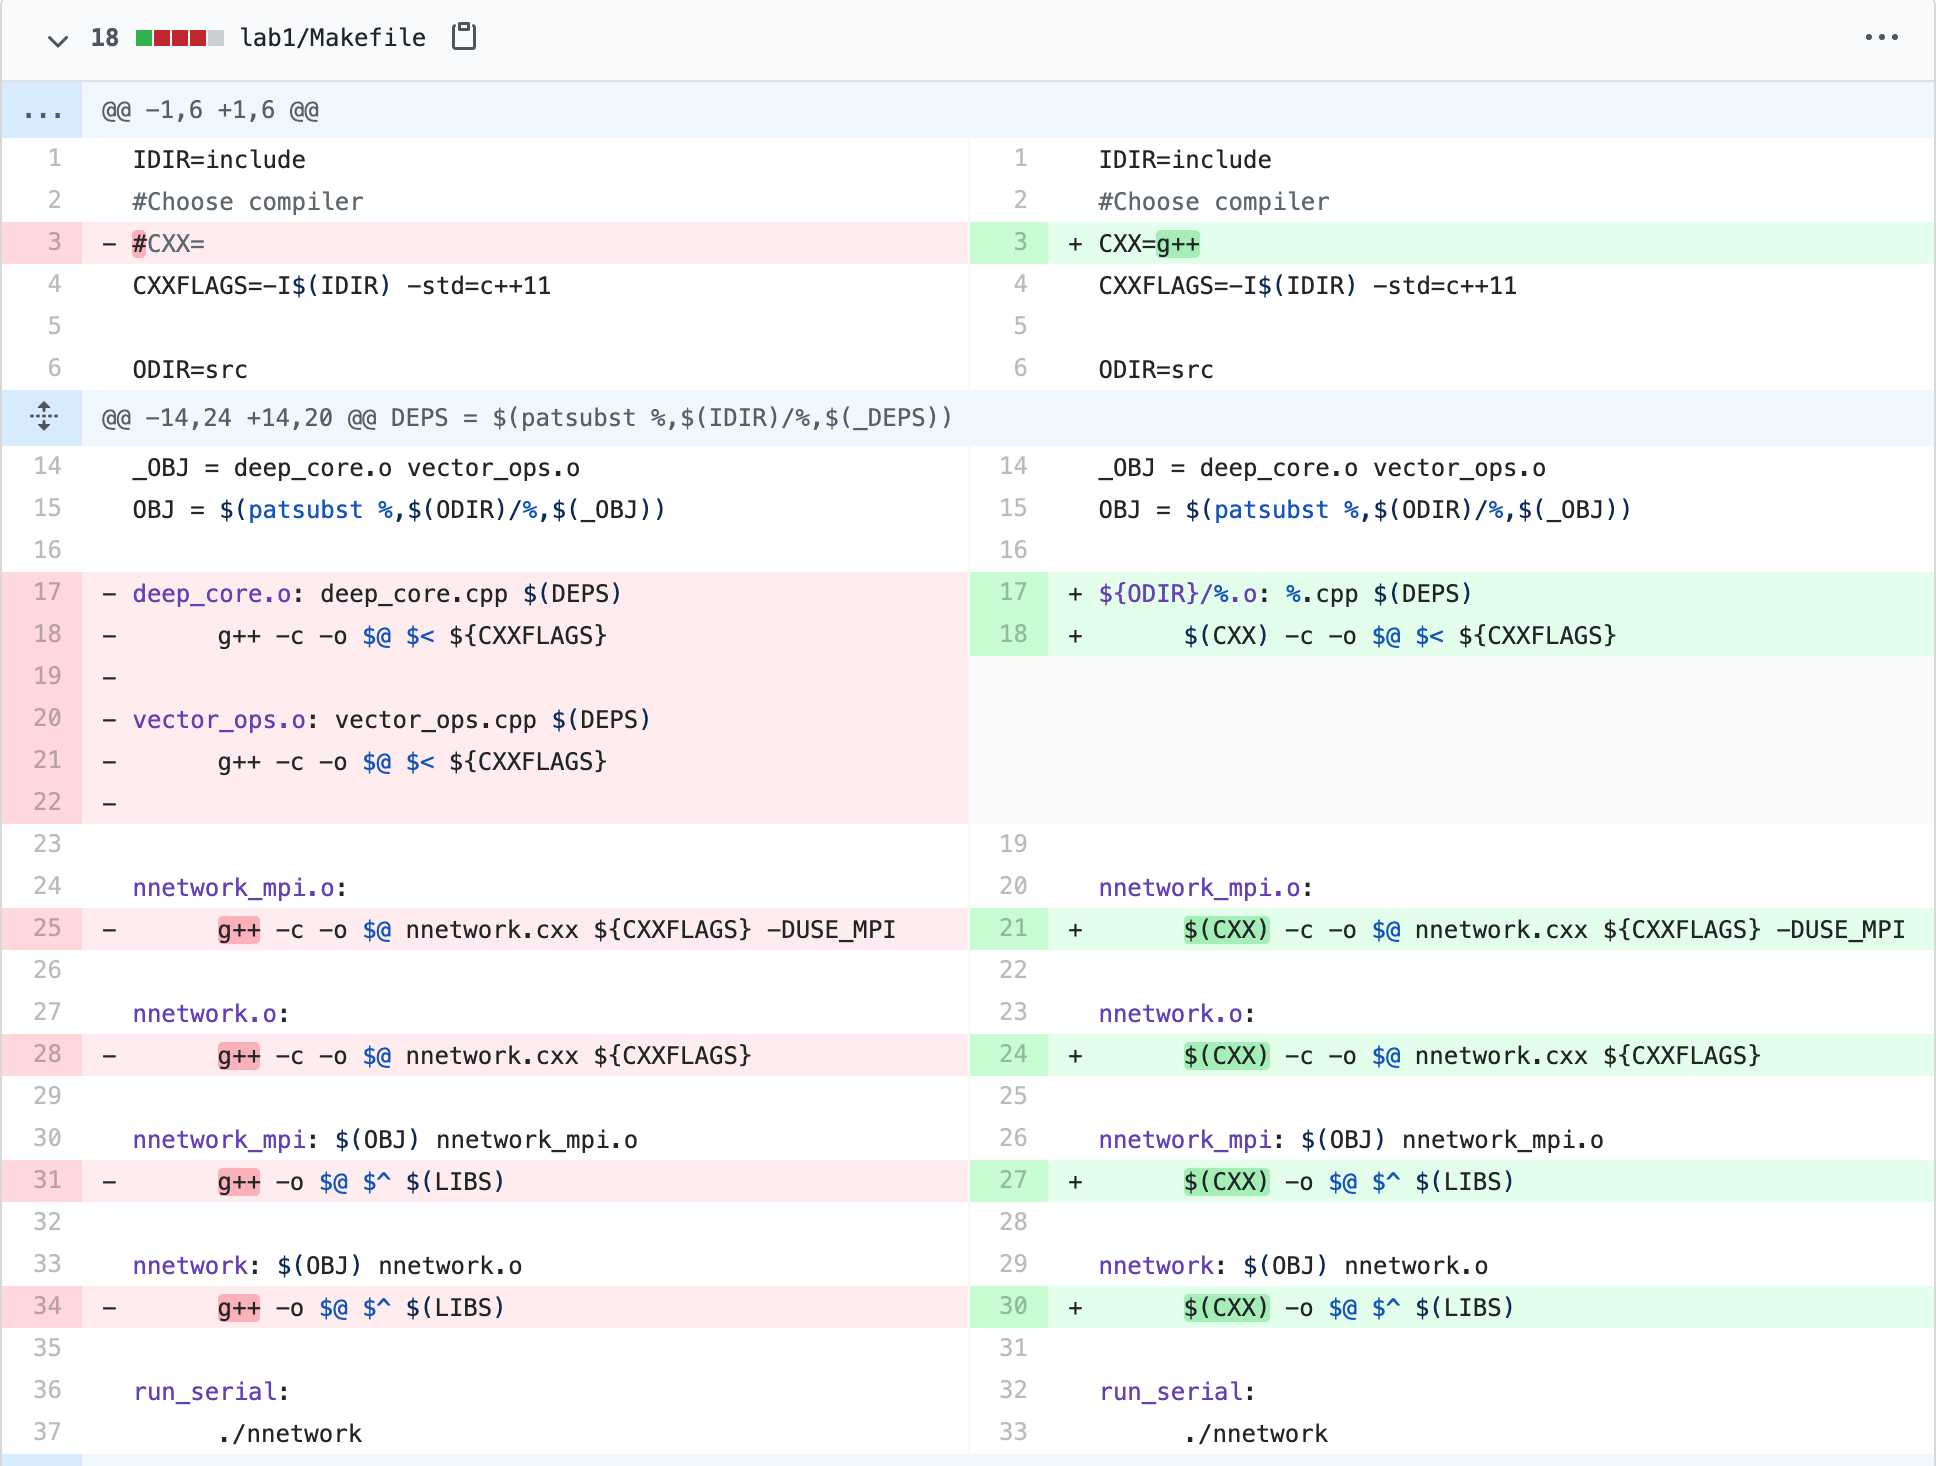
\includegraphics[scale=0.3]{task1 diff.png}
\end{center}

\subsection*{Task 2}
\begin{enumerate}[label=(\alph*)]
\item Make debug build:
\begin{center}
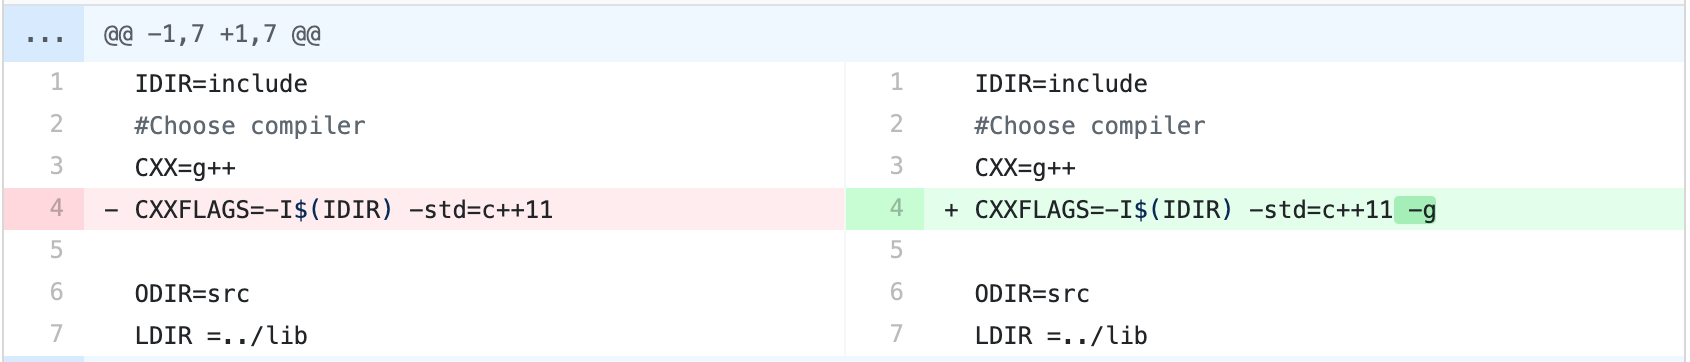
\includegraphics[scale=0.25]{task2.1.png}
\end{center}

\item Fix segfault:
\begin{center}
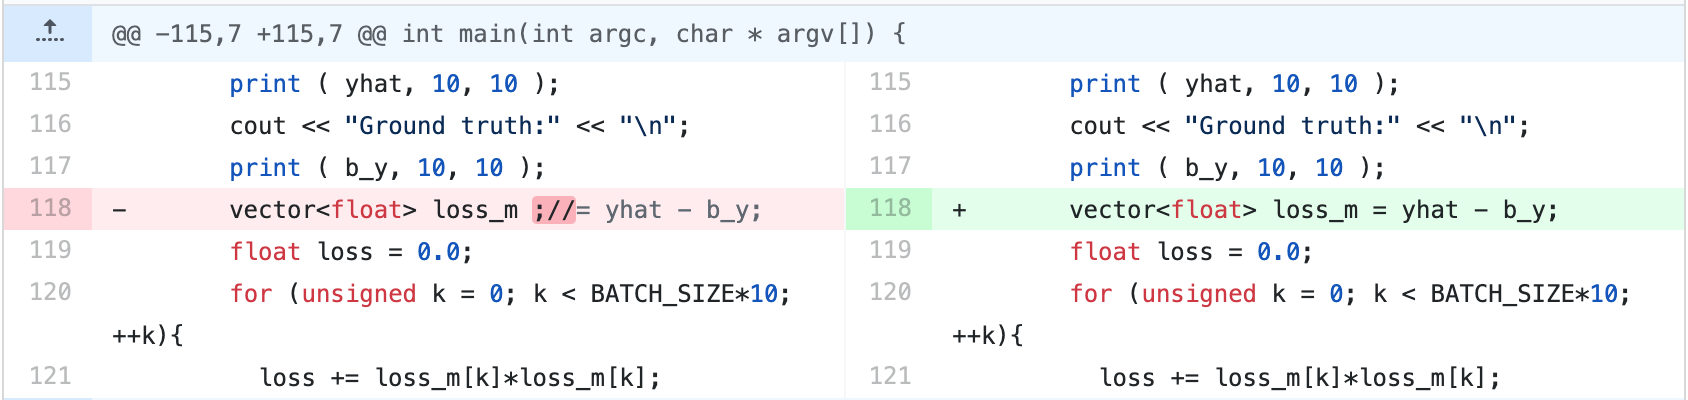
\includegraphics[scale=0.25]{task2.2.png}
\end{center}

\item After variable "size" is initialized, the value it contains is 32768. z is a const reference vector, containing floats.  z[3] = 1.96690202.
\begin{center}
	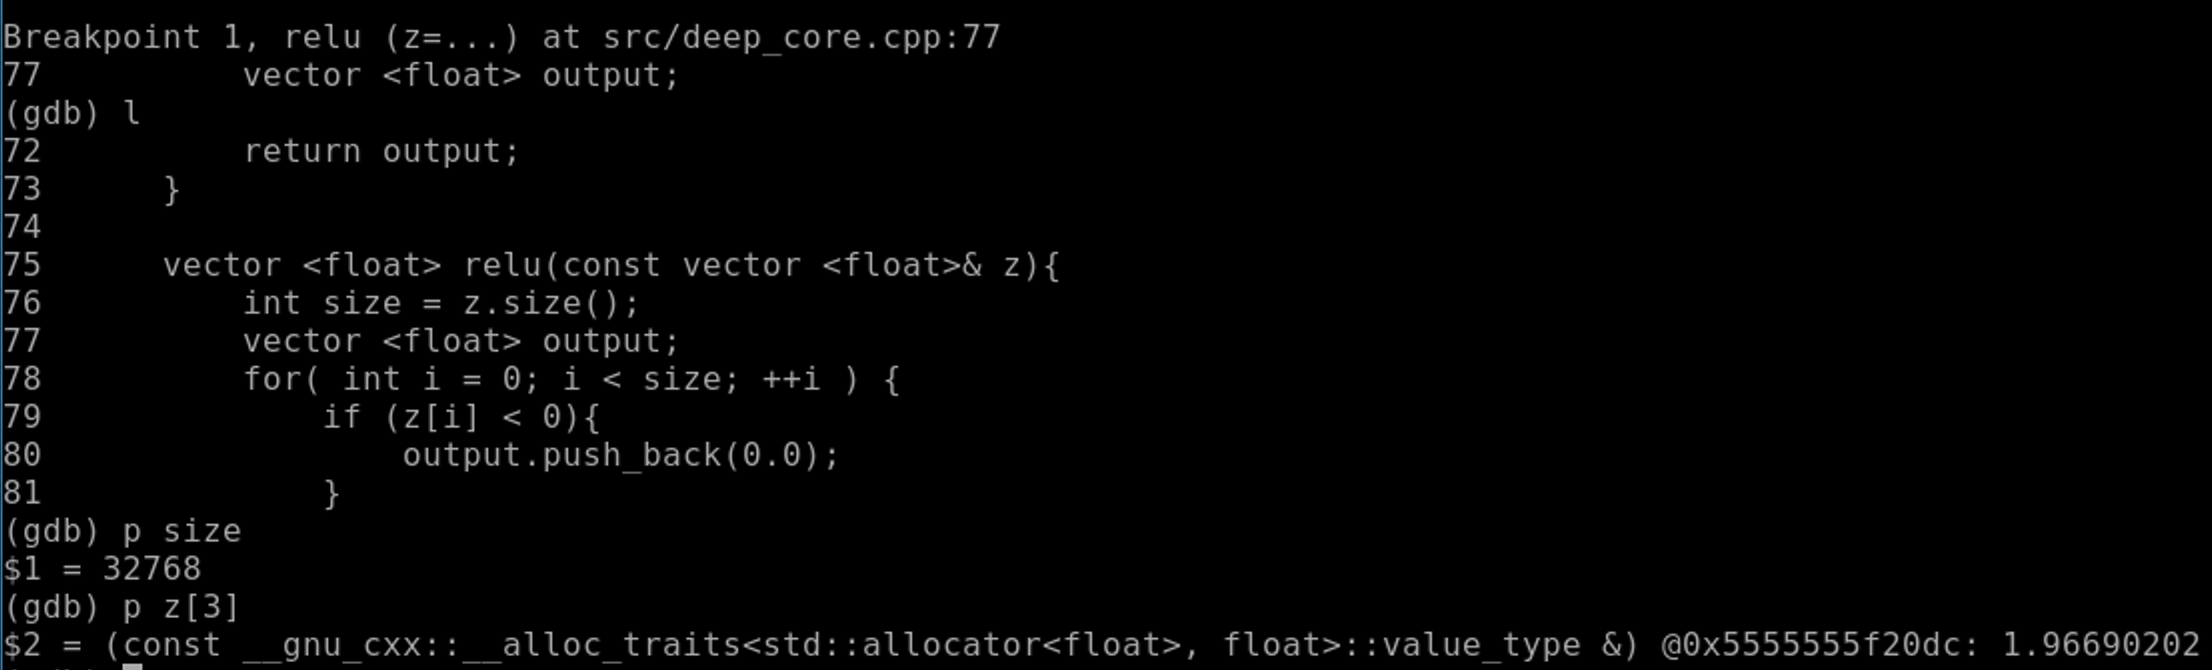
\includegraphics[scale=0.3]{task2.3.png}
\end{center}
\end{enumerate}

\subsection*{Task 3}
\begin{enumerate}[label=(\alph*)]
\item First, we have created a rule in the \textit{Makefile} to enable performance profiling. In particular, the rule is given by
\begin{verbatim}
run_perf:
    perf record ./nnetwork    .
\end{verbatim}

\item After running the added rule, we have inspected the generated performance file \texttt{perf.data} by running the command \texttt{perf report}. Overall, there are three time-consuming operations.
\begin{enumerate}[label=(\arabic*)]
\item The most time is spent in the \texttt{dot} function in the file \texttt{vector\_ops.cpp}. It requires about 67.62\% of running time and computes the product of two matrices. Optimizing it could highly improve the total running time of the training.
\item The second and third most time-consuming operations are array accesses on vector data-structures with 18.41\% and 9.36\% respectively. These operations might be optimized by reducing the number of cache misses while accessing vector elements.
\item Apart from those three operations, there are not any others with significant share on the running time. 
\end{enumerate}

\item To monitor the number of LLC cache misses, we have run the command \texttt{perf stat -e LLC-load-misses ./nnetwork}. However, the machine that we have been using did not support for that. The program returned
\begin{verbatim}
 Performance counter stats for './nnetwork':

         2,043,328      LLC-load-misses:u

     215.866059446 seconds time elapsed

     215.823836000 seconds user
       0.035999000 seconds sys

\end{verbatim}

\end{enumerate}

\end{document}
